\documentclass{article}
\usepackage{graphicx}
\usepackage{setspace}
% \usepackage{authblk}
\usepackage{url}
\usepackage[inline,shortlabels]{enumitem}
\usepackage[square,numbers]{natbib}
\usepackage{floatrow}
\floatsetup[table]{capposition=top}
\usepackage[nomarkers,nolists]{endfloat}
\usepackage[margin=1in,letterpaper]{geometry}
\usepackage{multirow}
\usepackage[table]{xcolor}
\usepackage[hidelinks]{hyperref}
\usepackage{lineno}
\linenumbers

\bibliographystyle{unsrtnat}

\begin{document}

\title{Supplementary Material}
\date{\vspace{-5ex}}

\maketitle

\doublespacing

\section{Optimizing default parameters}

We tried a number of parameter optimizations to set reasonable defaults.
We list them below and further discuss the bolded items.

\paragraph{Things that helped}

\begin{enumerate}
	\item \textbf{Adjust autoencoder depth}
	\item \textbf{Adjust discriminator depth}
	\item \textbf{Scale to [0, 1] with sigmoid}
	\item Make code layer more narrow
	\item Optimizing cross-entropy instead of MSE - trains faster
	\item Adjusting the lambda value - somewhat dataset specific
	\item Variational instead of normal autoencoder - loss is less erratic
	\item Dropout in the discriminator - less overfitting
\end{enumerate}

\paragraph{Things that didn't help}

\begin{enumerate}
	\item ReLU vs SELU \cite{klambauer_self-normalizing_2017} activation - no difference
	\item Recurrent discriminator connections - no difference
	\item Recurrent autoencoder connections (like UNet) - no difference
	\item Training autoencoder, discriminator, then dual optimizers sequentially - did worse
	\item Stopping early - did worse
\end{enumerate}

\paragraph{Adjust autoencoder depth}

\begin{figure}
	\centering
	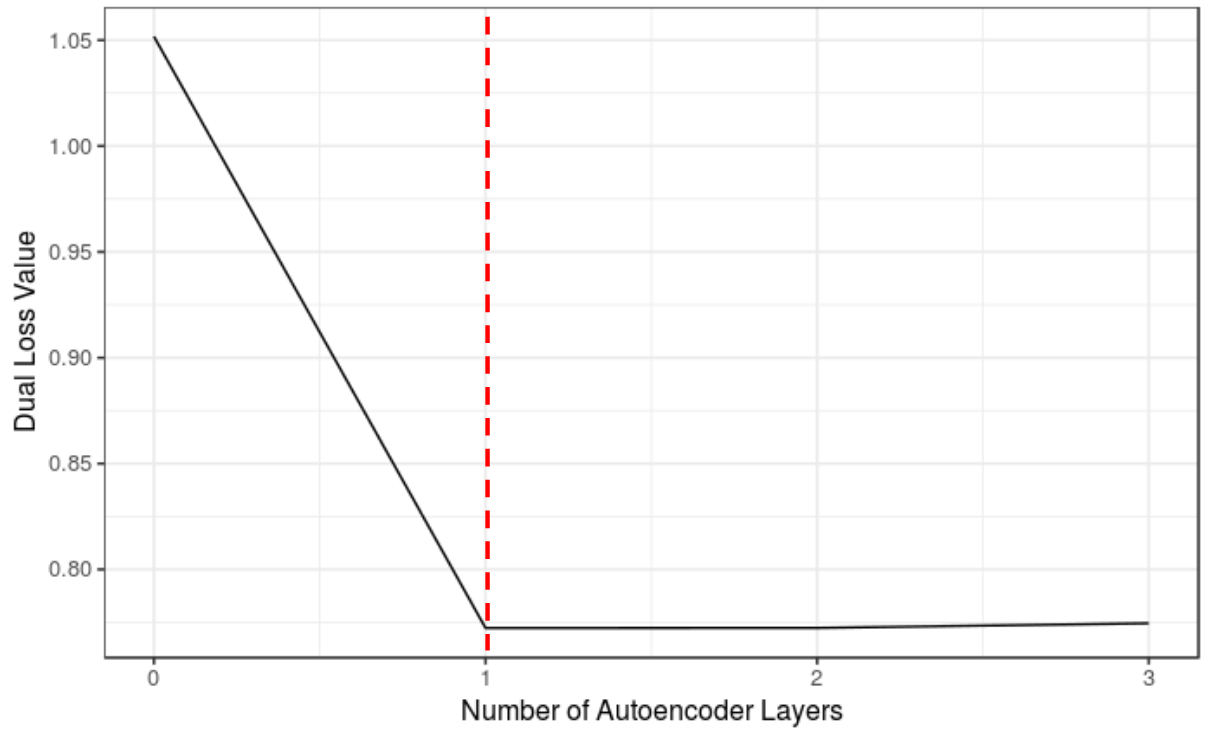
\includegraphics[width=\columnwidth]{figures/supplement/ae_layers.png}
	\caption{\textbf{Loss vs. Number of Autoencoder Layers}
	}
	\label{fig:ae}
\end{figure}

In order to prevent overfitting while allowing sufficient complexity for identifying and removing higher-order batch effects we added dropout to all the layers with a probability of 50\%.
We tested this autoencoder with varying encoding and decoding layer sizes in order to determine the optimal balance of complexity and speed.
We also tested several variations on autoencoders; we implemented a variation on the U-Net \cite{ronneberger_u-net_2015} and plan to test the network with a variational autoencoder \cite{kingma_auto-encoding_2013}.

\paragraph{Adjust discriminator depth}

\begin{figure}
	\centering
	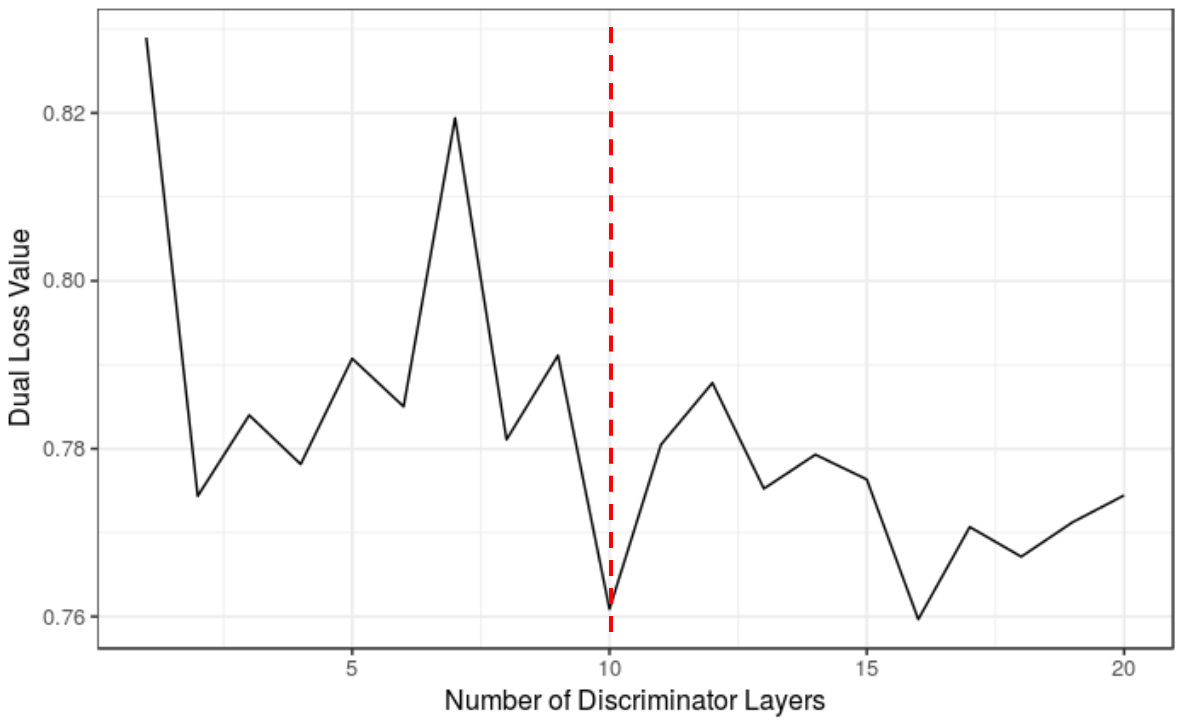
\includegraphics[width=\columnwidth]{figures/supplement/disc_layers.png}
	\caption{\textbf{Loss vs. Number of Discriminator Layers}
	}
	\label{fig:disc}
\end{figure}

We noticed that the discriminator was overfitting on the data.
Since it memorized which sample belonged to which batch instead of learning batch-specific patterns, the only way for the autoencoder to fool the discriminator was to completely obfuscate the expression data, therefore also removing any relevant signal.

\paragraph{Scale to [0, 1] with sigmoid}

\begin{figure}
	\centering
	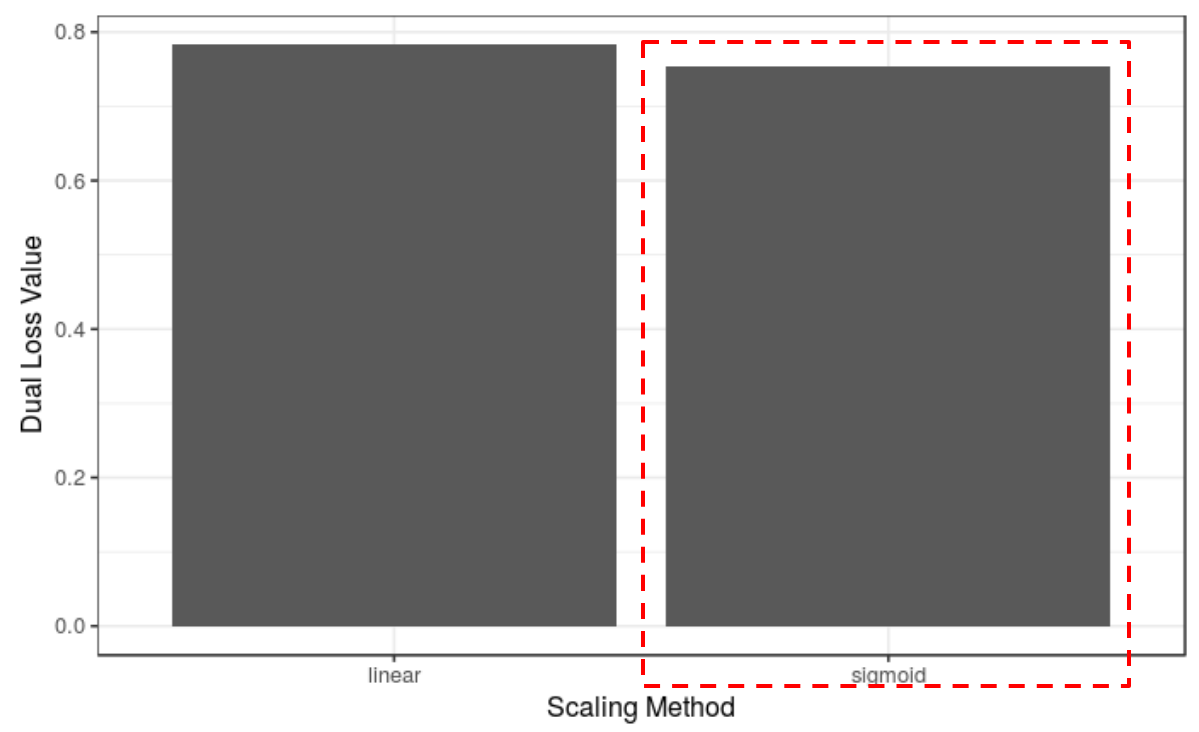
\includegraphics[width=\columnwidth]{figures/supplement/scaling.png}
	\caption{\textbf{Loss vs. Scaling Method}
	}
	\label{fig:scaling}
\end{figure}



\paragraph{Other ideas}

We toyed with the idea of using convolutional layers \cite{krizhevsky_imagenet_2012-1} in the network because of their incredible success in the realm of image recognition.
We thought at first that a 20,000-dimensional vector of expression values was quite similar to a 200x100 image and that similar techniques could be used for both, which was encouraging because convolutional filters are quite efficient for processing images.
However, we were unable to devise a representation or arrangement of gene expression data points in which convolutional filters would make sense.
Although one could easily wrap a gene expression vector into two dimensions and arrange the genes by location in the genome, each data point fundamentally represents a completely different gene product.
Contrast this with image data, where each pixel represents the same data type (i.e. relative light intensities of some wavelength); if each pixel value was shifted to the left by one pixel, the image would still represent the same idea.
However, if each expression value were to be shifted one position to the left, it would in essence be like mistaking each gene product for another unrelated gene product.
Therefore, passing convolutional filters over a gene expression array, 1D or 2D, would not make sense since the relationship between a pair of consecutive genes is not necessarily analogous to the relationship between another pair of consecutive genes.
Because we couldn't justify any arrangement where spatial relationships between genes were consistently meaningful, we chose to only use fully connected layers in Confounded rather than convolutional layers.
We welcome any future intellectual advances that may allow convolutional networks and other image processing techniques to be applied to expression data.

\paragraph{Datasets}

Working with each new dataset enlightened us of a new edge case that hadn't yet been addressed in our code.
By applying to our methods to each of the following datasets, our code became much more robust than if we had only developed and tested on one or two toy datasets.


\section{Data Format}

Confounded takes input data in the tidy data format \cite{wickham_tidy_2014-1}, namely:

\begin{itemize}
	\item Each row represents a different sample.
	\item Each column represents a different variable (either a clinical variable or a gene's expression).
\end{itemize}

Confounded parses through files in this format to determine which columns are discrete (integer or string) and which are continuous (floating point).
Each continuous column is interpreted to be a gene expression column and is adjusted for by the network according to the batch column.
This is one limitation to our software.
In a future iteration, it would be more robust to allow the user to specify continuous columns that should not be interpreted as gene expression data (e.g. ages in years with decimal precision representing fractions of years).
However for the datasets we tested, this didn't prove to be a problem.

\paragraph{GSE37199}

Additionally, this dataset has two levels of batches (``centre'' and ``plate'').
We identified this as an item of potential interest: can Confounded adjust for multiple batch effects simultaneously?
However, we left this question for future research and chose instead to focus on the ``plate'' effect for the time being.

\section{Testing different-sized datasets}

\begin{figure}
	\centering
	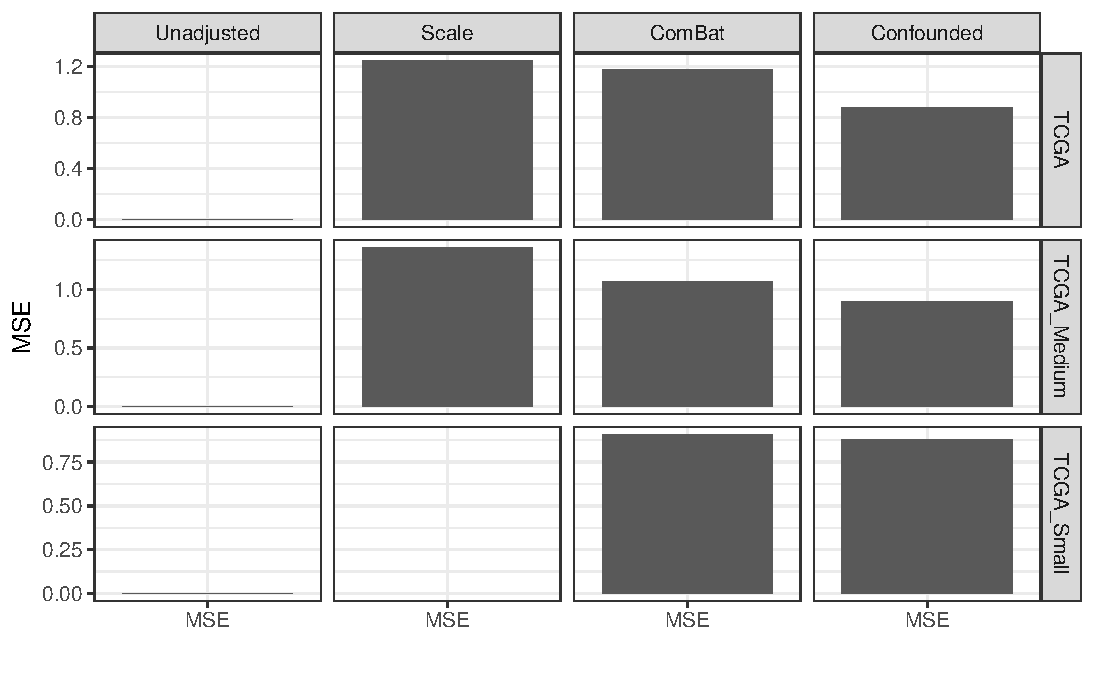
\includegraphics[width=\columnwidth]{figures/supplement/tcga_mse.pdf}
	\caption{\textbf{TCGA MSE}
	}
	\label{fig:mse}
\end{figure}
\begin{figure}
	\centering
	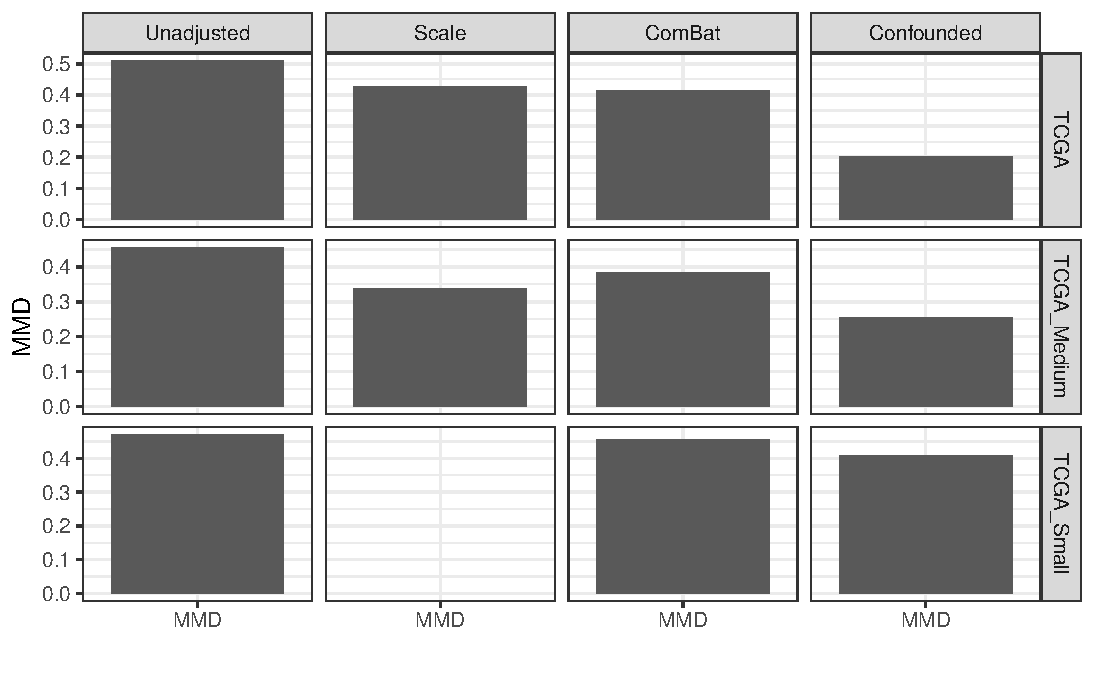
\includegraphics[width=\columnwidth]{figures/supplement/tcga_mmd.pdf}
	\caption{\textbf{TCGA MMD}
	}
	\label{fig:mmd}
\end{figure}
\begin{figure}
	\centering
	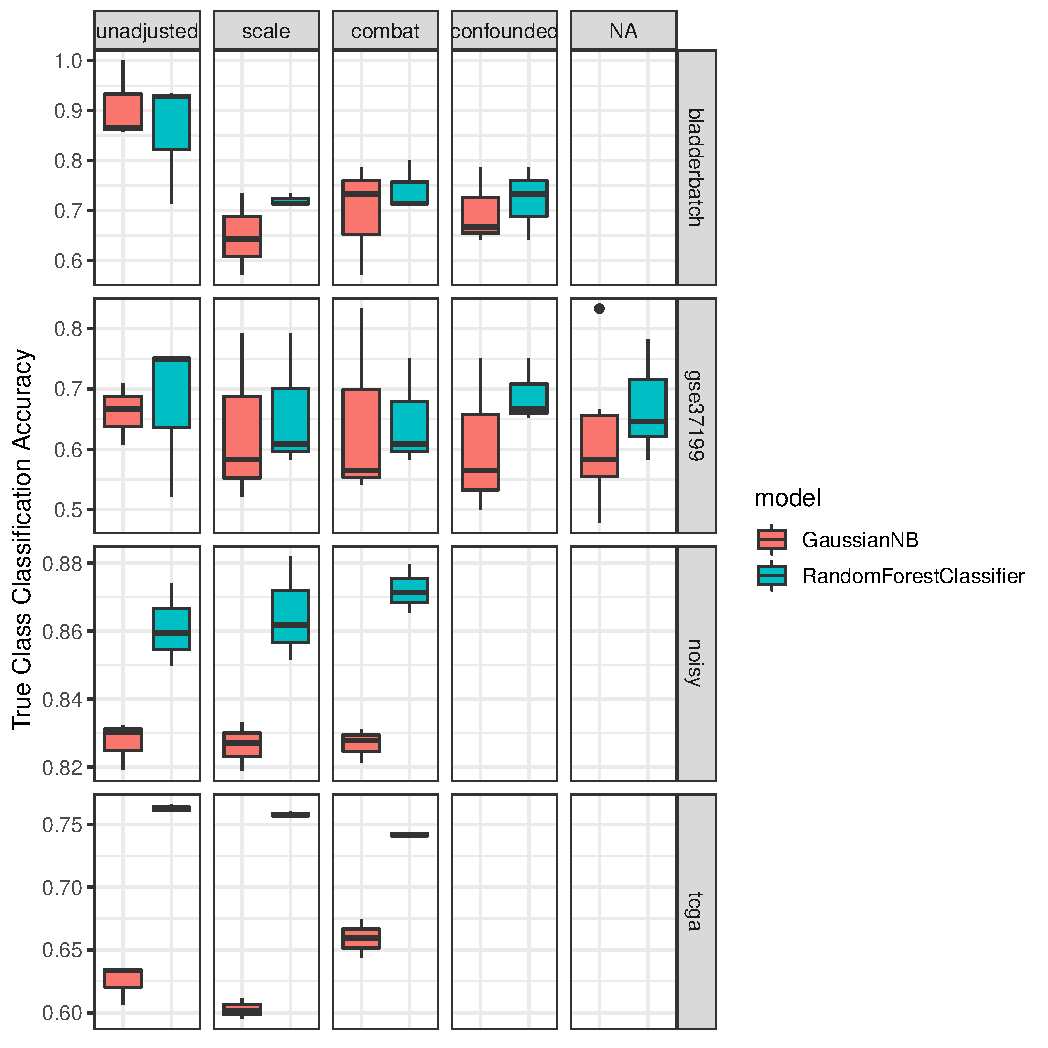
\includegraphics[width=\columnwidth]{figures/supplement/tcga_true_class_accuracy.pdf}
	\caption{\textbf{TCGA True Class Accuracy}
	}
	\label{fig:true_class}
\end{figure}
\begin{figure}
	\centering
	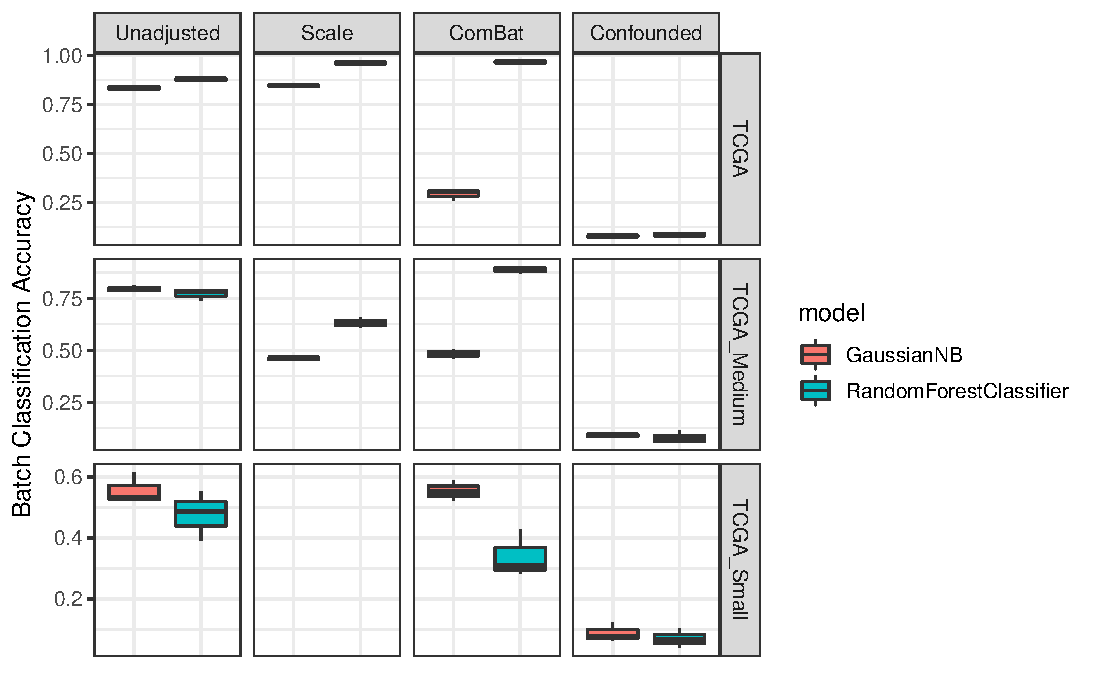
\includegraphics[width=\columnwidth]{figures/supplement/tcga_batch_accuracy.pdf}
	\caption{\textbf{TCGA Batch Accuracy}
	}
	\label{fig:batch}
\end{figure}

\section{Other methods}

We wanted to also compare with SVA \cite{leek_capturing_2007} and the Shaham lab's work \cite{shaham_removal_2017,shaham_batch_2018} but were unable to get these two methods to work.
With SVA, the documentation showed how to identify surrogate variables and use them in modeling, but we were unable to find examples of removing the effects that those surrogate variables represent.
We were unable to get the Shaham lab's methods running on our datasets, and we believe that this is due to some underlying assumptions in their code.

\section{Metrics used}

\paragraph{MSE}

We calculate MSE by the following:

\begin{equation}
	\label{mse}
	MSE = \frac{1}{n}\sum_{i=1}^n{(\hat{x}_i - x_i)^2}
\end{equation}

Where $x$ represents the values in the autoencoder's input and $\hat{x}$ represents the approximated values in the output.
If $x = \hat{x}$, MSE will be 0.

\paragraph{MMD}

We wanted to compare our network against this network, so we calculated MMD for each adjuster.
Unfortunately, we were unable to get their network to work on our datasets for comparison due to some assumptions in their code (there must only be two batches, the two batches must be perfectly balanced, and the dataset must be fairly large).

following formula:

\begin{equation}
	\label{mmd}
	MMD(x, y) = \frac{1}{n^2}\sum_{i=1}^n{\sum_{j=1}^n{k(x_i, x_j)}} - \frac{2}{nm}\sum_{i=1}^n{\sum_{j=1}^m{k(x_i, y_j)}} + \frac{1}{m^2}\sum_{i=1}^m{\sum_{j=1}^m{k(y_i, y_j)}}
\end{equation}

Where $k(x, y)$ is the Gaussian kernel between $x$ and $y$ as implemented in \texttt{sklearn.metrics.pairwise.rbf\_kernel}, and where $x$ represents the data from one batch and $y$ represents the data from another batch.
In cases where there were more than two batches (e.g. $x$, $y$, and $z$), we averaged the pairwise MMD values to calculate an overall MMD:

\begin{equation}
	\label{mmd-mean}
	MMD_{total}(x, y, z) = \frac{1}{3}[MMD(x, y) + MMD(x, z) + MMD(y, z)]
\end{equation}
% TODO: make this formula ^ apply to more than 3 batches

\paragraph{PCA \& t-SNE}

\begin{figure}
	\centering
	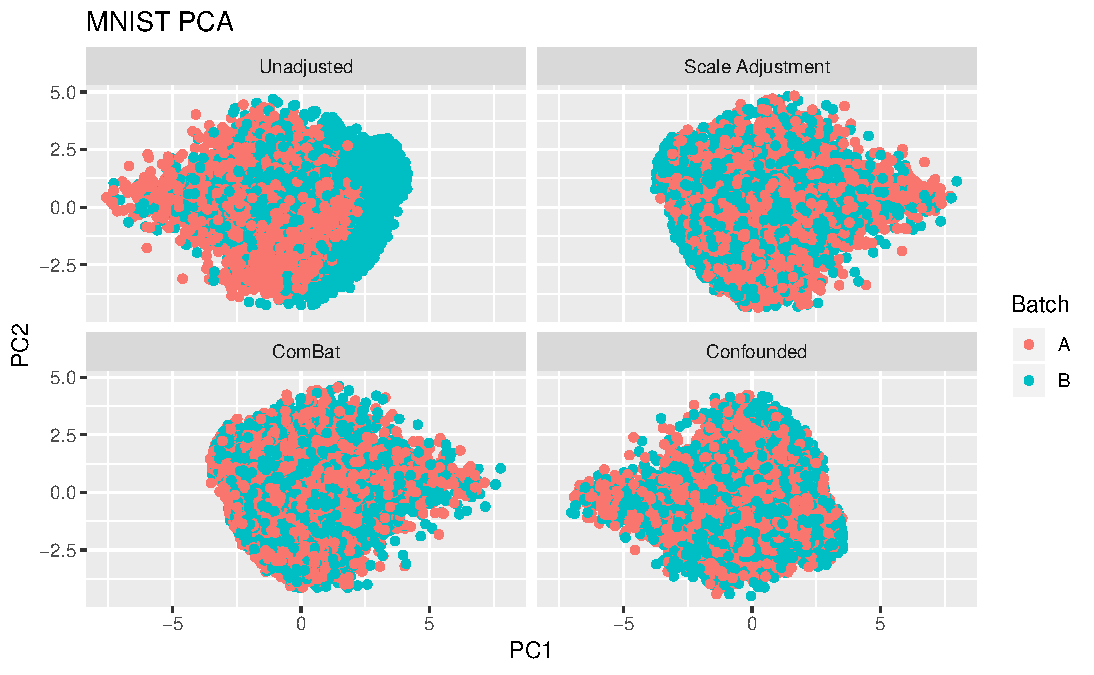
\includegraphics[width=\columnwidth]{figures/supplement/mnist_pca.pdf}
	\caption{\textbf{MNIST PCA}
	}
	\label{fig:pca}
\end{figure}
\begin{figure}
	\centering
	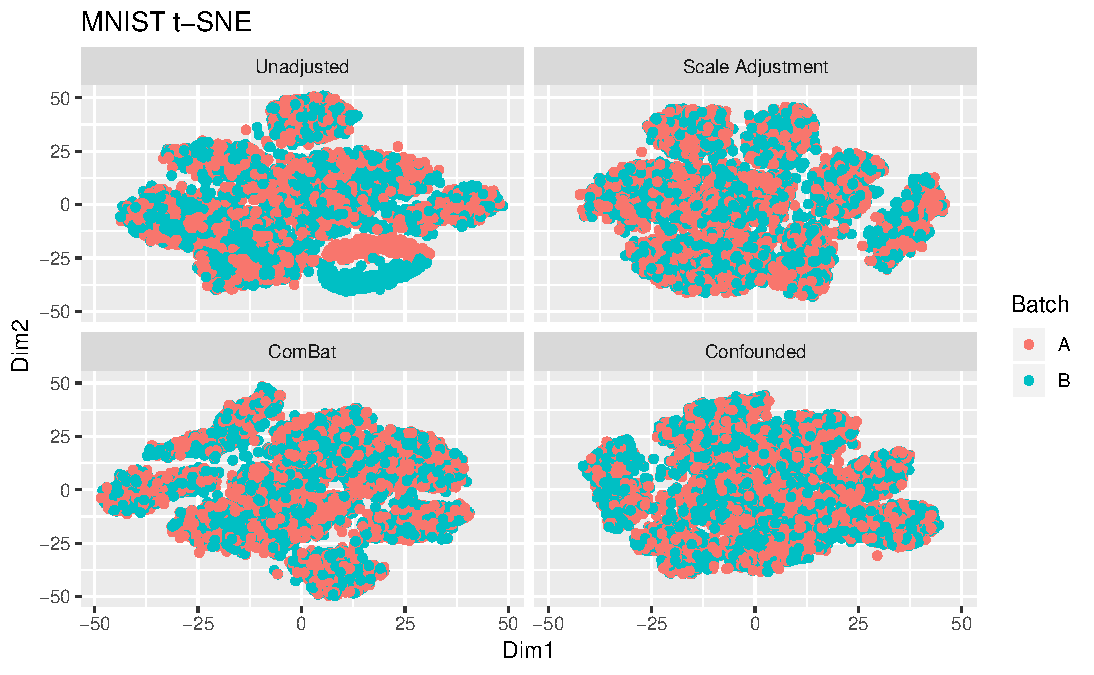
\includegraphics[width=\columnwidth]{figures/supplement/mnist_tsne.pdf}
	\caption{\textbf{MNIST t-SNE}
	}
	\label{fig:tsne}
\end{figure}

\bibliography{references}

\end{document}
